\chapter{Spin torque oscillators} \label{chap:STO}
In this chapter we will cover the second topic of this thesis, which is spin torque oscillators. These oscillators are realized by a magnetic multilayer system, where the free magnetic moments in the system can undergo self-sustained oscillations. Due to the giant magnetoresistance effect this causes a temporally varying resistance of a current passing through the multilayer system, allowing us to generate an alternating current by applying a direct current to the system. Like the magnetization dynamics of the skyrmion, these self-sustained oscillations can be described by a variation of the LLG equation, known as the Landau--Lifshitz--Gilbert--Slonczewski (LLGS) equation. Because of the geometry of the multilayer system, it is possible to induce a Rashba spin--orbit coupling due to the broken inversion symmetry. The effect of this spin--orbit coupling on the spin torque oscillator in such a multilayer system has to date not yet been explored, and is the purpose of this chapter. We will in this chapter perform analytical and numerical calculations on the system when RSOC is present, and find an analogous description of this effect comparing it to well known effects.

\section{Giant magnetoresistance}
An important effect that is fundamental for the spin torque oscillators is the giant magnetoresistance (GMR) effect. This effect was discovered by Albert Fert \cite{Fert1988} and Peter Gr\"{u}nberg \cite{Grunberg1989} in 1988, for which they won the Nobel prize in 2007. They discovered that when an electrical current passed through a layered magnetic system with different magnetic orientations, the resistance changed considerably depending on whether the magnetic layers were parallel or anti-parallel, as illustrated in Figure \ref{fig:GMR}. The reason for this difference in resistance is that electrons with magnetic moments aligned with the local magnetization are scattered far less than electrons that have a component in their magnetic moments that is perpendicular to the local magnetization \cite{Chappert2007}. This can be argued through the fact that in the ferromagnetic coupling between the itinerant and local electrons, the electrons that are not aligned with the local magnetization have a higher exchange energy than electrons that are aligned. They then have to pass through a higher energy barrier than the aligned electrons, and the current of those electrons will therefore have a higher resistance.
\begin{figure}[h!]
\centering
  \begin{subfigure}[b]{.58\textwidth}
  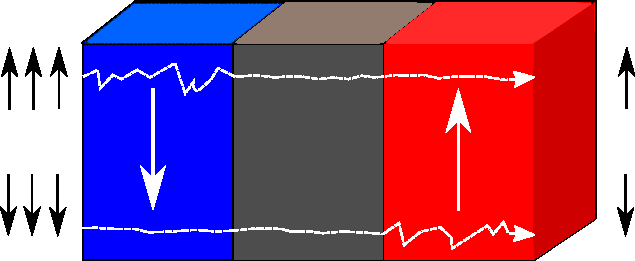
\includegraphics[width=\linewidth]{Figures/GMR_APv2.pdf}
  \caption{}
  \label{fig:GMR_AP}
\end{subfigure}
\begin{subfigure}[b]{.6\textwidth}
  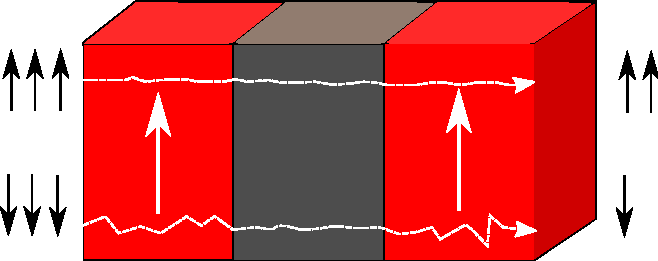
\includegraphics[width=\linewidth]{Figures/GMR_Pv2.pdf}
  \caption{}
  \label{fig:GMR_P}
\end{subfigure}
\caption{The resistance of a current passing through a multilayered magnetic system depends on the magnetic moment of the electron (proportional to their spin) and the alignment of the magnetic layers. Here we consider an anti-parallel configuration in \textbf{(a)} and a parallel configuration in \textbf{(b)} separated by a non-magnetic material. In \textbf{(a)} the resistance is high because of the anti-parallel configuration of the magnetic layers the current has to pass through, leading to considerable scattering of the anti-parallel magnetic moments of the electrons. In \textbf{(b)} the resistance of the electrons with a magnetic moment parallel to the magnetic layers is lower than the electrons with an anti-parallel magnetic moment.}
\label{fig:GMR}
\end{figure}

GMR has most noticeably been utilized in nonvolatile memory technologies such as magnetoresistive random-access memory (MRAM) \cite{Akerman2005} and racetrack memories \cite{Parkin2008}. The GMR is pivotal in spin torque oscillators, as the resistance is a function of the angle between two magnetizations. If we were able to make these magnetizations oscillate, such that the angle between them varies in time, the oscillation in the resistance due to GMR will cause an oscillation in the current. We would then have an oscillator that converts the direct current applied to the system into an alternating current. This type of system that utilizes the precession of magnetic moments to generate an oscillating current is known as a spin torque oscillator (STO).

\section{Spin torque oscillators under influence of spin--orbit coupling}
The spin torque oscillators that we will consider in this thesis primarily consist of a fixed polarizing magnetic layer, and two free magnetic layers that interact with each other through the RKKY interaction. We will study the effects the Rashba spin--orbit coupling may have in two different geometries, a bulk geometry and a thin film geometry, as illustrated in Figure \ref{fig:Geometries}. Whether the system is in an oscillating state depends on the system parameters, such as the strength of the magnetic anisotropy (which we assume to be uniaxial), the current density inducing spin-transfer torques, and the strength of the RKKY interaction between the free magnetic layers. Spin torque oscillators have been found to occur in both ferromagnetic \cite{Zhou2013} and antiferromagnetic \cite{Klein2012} coupling between the free magnetic layers. By varying some of these parameters we can study when the system is in an STO phase, or when a collinear state where the free magnetic layers are aligned or anti-aligned with the easy axis of the material is stable. This would result in a phase diagram that would give information regarding what state we will find the system in for a given set of parameters. The goal of this chapter is to study the effects of Rashba spin--orbit coupling on the STO phase in this phase diagram, and the effects it has on the oscillation frequency of the current going out of the system. 
\begin{figure}[h!]
\centering
%\begin{center}
\begin{subfigure}{.6\textwidth}
  \begin{tikzpicture}
\node[above right] (img) at (0,0) {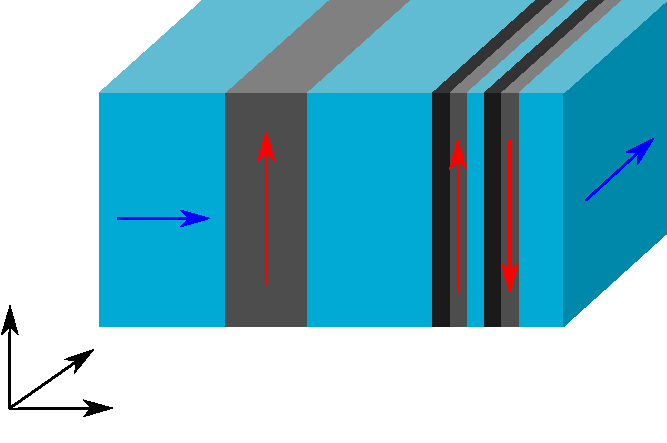
\includegraphics[width=1\textwidth]{Figures/STO_Bulkv2}};
\node at (10pt,70pt) {\Large{$z$}};
\node at (32pt,47pt) {\Large{$y$}};
\node at (42pt,8pt) {\Large{$x$}};
\node at (115pt,40pt) {\Large{F$_0$}};
\node at (192pt,40pt) {\Large{F$_1$}};
\node at (215pt,40pt) {\Large{F$_2$}};
\node at (70pt,110pt) {\textcolor{blue}{\Large{$\mathbold{j}_x$}}};
\node at (255pt,130pt) {\textcolor{blue}{\Large{$\mathbold{j}_y$}}};
\end{tikzpicture}
\caption{}
\label{fig:BulkGeometry} 
\end{subfigure}

\begin{subfigure}{.6\textwidth}
  \begin{tikzpicture}
\node[above right] (img) at (0,0) {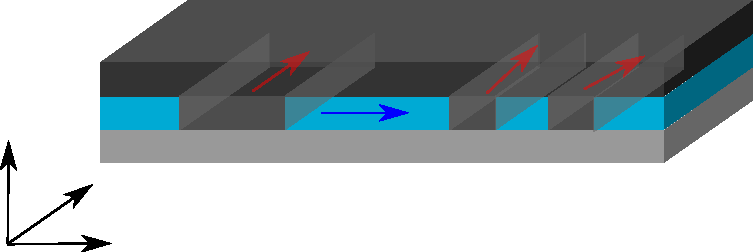
\includegraphics[width=1\textwidth]{Figures/STO_Filmv2}};
\node at (8pt,50pt) {\Large{$z$}};
\node at (28pt,32pt) {\Large{$y$}};
\node at (37pt,-2pt) {\Large{$x$}};
\node at (90pt,25pt) {\Large{F$_0$}};
\node at (177pt,25pt) {\Large{F$_1$}};
\node at (212pt,25pt) {\Large{F$_2$}};
\node at (160pt,54pt) {\textcolor{blue}{\large{$\mathbold{j}_x$}}};
\end{tikzpicture}
\caption{}
\label{fig:FGeometry} 
\end{subfigure}
%\end{center}
\caption{Illustrations of \textbf{(a)} the bulk geometry and \textbf{(b)} the thin film geometry. In geometries a fixed magnetic layer F$_0$ is separated from two free magnetic layers F$_1$ and F$_2$ by a non-magnetic metallic material shown here in blue. A material illustrated in black, which is neighboring to F$_1$ and F$_2$ in \textbf{(a)} and the top film in \textbf{(b)}, is present to get a strong Rashba spin--orbit coupling at the interface of the free ferromagnetic layers. In \textbf{(b)} the bottom film is a material that will cause little to no RSOC at the interface to the ferromagnetic materials. To induce dynamics a current is applied in the $x$-direction which causes $\mathbold{m}_1$ and $\mathbold{m}_2$ to experience spin-transfer torques. In \textbf{(a)} a current is also applied in the $y$-direction to create significant RSOC effects on $\mathbold{m}_1$ and $\mathbold{m}_2$ due to the symmetry breaking in the $x$-direction. In the film geometry this is caused by the current in the $x$-direction as the symmetry breaking is in the $z$-direction. The free magnetic layers also interact through the RKKY interaction, while the distance to the fixed magnetic layer is chosen such that an RKKY interaction with this layer can be neglected. In \textbf{(a)} the material has an easy axis in the $z$-direction, while in \textbf{(b)} the material has an easy axis in the $y$-direction.}
\label{fig:Geometries}
\end{figure}

The model that we will use to analyze this system is a variation of the Landau--Lifshitz--Gilbert--Slonczewski (LLGS) equation that includes the Rashba field derived by Kim \etal~\cite{Kim2012}. The LLGS equation is an expansion of the LLG equation \eqref{eq:LLG} that includes spin-transfer torques on uniform magnetic moments. Usually the non-adiabatic spin-transfer torque is rather small compared to the adiabatic spin-transfer torque, to an order of magnitude on the size of the Gilbert damping $\alpha$ (which is typically $~10^{-2}$ for the systems we will consider). This torque still has a significant contribution to the dynamics of the magnetization even at this order of magnitude, as we have previously seen in the skyrmion dynamics. In metallic multilayers such as N/F/N/F/N (N being a non-magnetic metal, and F being a ferromagnetic metal), however, the non-adiabatic STT is even smaller than usual due to symmetry considerations. The lowest contribution to the non-adiabatic STT in such a system becomes quadratic in the applied voltage bias $V$ that generates the current responsible for STT. Since the voltage bias necessary to generate large current densities for systems at this scale is quite small, a torque that is proportional to $V^2$ can be neglected. This symmetry consideration is discussed in more detail by Ralph and Stiles \cite{Ralph2008}. We are then content by only including the adiabatic spin-transfer torque in our model, and the LLGS equation that we consider then becomes
\begin{align}
    \label{eq:LLGS}
    \partial_t \mathbold{m}_i = -\gamma \mathbold{m}_i\times\left(\mathbold{H}^{\text{eff}}_i+\mathbold{H}^{\text{R}}_i - \beta\mathbold{m}_i\times\mathbold{H}^{\text{R}}_i\right) + \alpha\mathbold{m}_i \times\partial_t\mathbold{m}_i + \mathbold{T}^{\text{STT}}_i,
\end{align}
with $\mathbold{m}_i$ being the magnetization in F$_i$. We remember that the Rashba field is given by
\begin{align}
    \mathbold{H}^{\text{R}}_i = \frac{1}{1+\beta^2}\frac{\alpha_{\text{R}}m_e P(i) j}{e M_s \hbar \mu_0} \mathbold{\hat{n}}\times\mathbold{\hat{j}}.
\end{align}
The polarization $P(i)$ is the polarization of the current responsible for the spin--orbit coupling at the interface between F$_i$ and the material that induces a strong RSOC at the interface. Note that the non-adiabatic contribution of the Rashba field proportional to $\beta$ is still included, as the same symmetry argument that allowed us to neglect the non-adiabatic STT is not applicable to this torque. The adiabatic STT acting on $\mathbold{m}_1$ and $\mathbold{m}_2$ are given by
\begin{subequations}
\begin{align}
    \mathbold{T}^{\text{STT}}_1 &= -\frac{\gamma \hbar j_x}{2 e M_s \mu_0 d} \mathbold{m}_1\times\left( P_0\mathbold{m}_0 - P_1 \mathbold{m}_2\right) \times \mathbold{m}_1, \\
    \mathbold{T}^{\text{STT}}_2 &= -\frac{\gamma \hbar j_x}{2 e M_s \mu_0 d} P_1 \mathbold{m}_2\times \mathbold{m}_1 \times \mathbold{m}_2,
\end{align}
\end{subequations}
following the derivation in Section \ref{sec:AdSTT}. Here $P_i$ is the polarization of the current after having passed through F$_i$. The effective field $\mathbold{H}^{\text{eff}}_i$ in the free magnetic layer F$_i$ is given by the field resulting from magnetic anisotropy and the RKKY interaction, which becomes
\begin{align}
    \mathbold{H}^{\text{eff}}_i = \frac{2K}{\mu_0 M_s}\left( \mathbold{m}_i \cdot \mathbold{\hat{n}}_k\right)\mathbold{\hat{n}}_k + \frac{J_{\text{RKKY}}}{\mu_0 M_s d} \mathbold{m}_{\bar{i}}.
\end{align}
Here $\mathbold{\hat{n}}_k$ is a unit vector along the easy axis, $d$ is the thickness of the free magnetic layers F$_1$ and F$_2$ (which are assumed to have an equal thickness), and $\bar{i}$ indicates the index of the free magnetic layer that is not $i$ ($\bar{i} = 3 - i$). To study the different stable phases of this system, which we assume to be collinear states along $\mathbold{\hat{n}}_k$, we follow the derivation by Zhou \etal~\cite{Zhou2013}. We first make the ansatz that we have a small perturbation $\mathbold{u}_i$ from a collinear state, so that $\mathbold{m}_i \approx \lambda_i\mathbold{\hat{n}}_k + \mathbold{u}_i$, where $\lambda_i = \pm 1$. The possible collinear states in question are $\downarrow\downarrow, \downarrow\uparrow, \uparrow\downarrow, \uparrow\uparrow$, with the arrows indicating the direction of $\mathbold{m}_1$ and $\mathbold{m}_2$ respectively, and $\uparrow$ being the unit vector $\mathbold{\hat{n}}_k$ along the easy axis. To decide whether the collinear state is stable, we must study the time evolution of the perturbation $\mathbold{u}_i$. This is done by performing a Fourier transform of the LLGS equation using our ansatz of $\mathbold{m}_i$, which is shown in Appendix \ref{app:FourierLLGS}. The end result can be written compactly as
\begin{align}
    \label{eq:EigenvalueEqn}
    \left(\hat{A}\omega + \hat{V}\right)
    \begin{pmatrix}
     \tilde{\mathbold{u}}_1 \\
     \tilde{\mathbold{u}}_2
    \end{pmatrix}
    = 0.
\end{align}
The matrices for the different geometries are given by
\begin{subequations}
\begin{align}
    \hat{A}_{\text{bulk}} &=
    \begin{pmatrix}
     1-i\alpha\lambda_1 & 0 \\
     0 & 1-i\alpha\lambda_2
    \end{pmatrix}, \label{eq:Abulk}\\
    \hat{A}_{\text{film}} &=
    \begin{pmatrix}
     1+i\alpha\lambda_1 & 0 \\
     0 & 1+i\alpha\lambda_2
    \end{pmatrix}, \label{eq:Afilm}\\
    \nonumber\hat{V}_{\text{bulk}} &=
    \omega_0\begin{pmatrix}
     \lambda_1 & 0 \\
     0 & \lambda_2
    \end{pmatrix}
    + \omega_J \begin{pmatrix}
     \lambda_2 & -\lambda_1 \\
     -\lambda_2 & \lambda_1
    \end{pmatrix}
    + i\omega_j^{(x)}\left[P_0
    \begin{pmatrix}
     -\lambda_1 & 0 \\
     0 & 0
    \end{pmatrix}
    + P_1
    \begin{pmatrix}
     \lambda_1\lambda_2 & -1 \\
     1 & -\lambda_1\lambda_2
    \end{pmatrix}\right] \\
    &\hspace{4.5mm} \frac{\omega_R^{(y)}}{1+\beta^2}\left[
    \begin{pmatrix}
     P_1^{(y)} & 0 \\
     0 & P_2^{(y)}
    \end{pmatrix}
    - i \beta
    \begin{pmatrix}
     P_1^{(y)}\lambda_1 & 0 \\
     0 & P_2^{(y)}\lambda_2
    \end{pmatrix}\right], \label{eq:Vbulk}\\
    \nonumber\hat{V}_{\text{film}} &=
    -\omega_0\begin{pmatrix}
     \lambda_1 & 0 \\
     0 & \lambda_2
    \end{pmatrix}
    - \omega_J \begin{pmatrix}
     \lambda_2 & -\lambda_1 \\
     -\lambda_2 & \lambda_1
    \end{pmatrix}
    + i\omega_j^{(x)}\left[P_0
    \begin{pmatrix}
     -\lambda_1 & 0 \\
     0 & 0
    \end{pmatrix}
    + P_1
    \begin{pmatrix}
     \lambda_1\lambda_2 & -1 \\
     1 & -\lambda_1\lambda_2
    \end{pmatrix}\right] \\
    &\hspace{4.5mm} -\frac{\omega_R^{(x)}}{1+\beta^2}\left[
    \begin{pmatrix}
     P_0 & 0 \\
     0 & P_1
    \end{pmatrix}
    + i \beta
    \begin{pmatrix}
     P_0\lambda_1 & 0 \\
     0 & P_1\lambda_2
    \end{pmatrix}\right]. \label{eq:Vfilm}
\end{align}
\end{subequations}
Here we have defined the frequencies $\omega_0 = 2\gamma K/\mu_0M_s$, $\omega_J = \gamma J_{\text{RKKY}}/\mu_0 M_s d$, $\omega_j^{(x)} = \gamma \hbar j_x/2\mu_0M_sd$ and $\omega_R^{(x/y)} = \gamma \alpha_R m_e j_{x/y}/\hbar\mu_0 e M_s$. $\tilde{\mathbold{u}}_1$ and $\tilde{\mathbold{u}}_2$ are the Fourier transforms of $\mathbold{u}_1$ and $\mathbold{u}_2$, and are defined as $\mathbold{u}_i(t) = \int \tilde{\mathbold{u}}_i(\omega) \exp\left(-i\omega t\right) \d \omega/{2\pi}$. From this definition we can see that the perturbation is stable when the imaginary part of $\omega$ is less than zero, but when the imaginary part of $\omega$ is greater than zero the perturbation is exponentially increasing. To determine the sign of the imaginary component of $\omega$ we use \eqref{eq:EigenvalueEqn}. By rearranging the terms and multiplying with the inverse of $\hat{A}$, we see that $\omega$ is restricted to be one of the two possible eigenvalues of the $2\times2$ matrix $\hat{W} = -\hat{A}^{-1}\hat{V}$. The collinear state $\mathbold{m}_1=\lambda_1\mathbold{\hat{n}}_k$, $\mathbold{m}_2=\lambda_2\mathbold{\hat{n}}_k$ is then stable if both of the eigenvalues of $\hat{W}$ have negative imaginary components. This is of course dependent on the system parameters. We can then use this matrix to find the phase diagrams for when the collinear states are stable or not. There will be a region where none of the collinear states are stable for some choice of parameters, and it is in this region that an STO phase will have to be localized. However, a lack of a stable collinear state does not indicate that we have an STO phase. Our analytical model can only describe if a perturbation from a collinear state will increase or relax back to its original state, and if the perturbation is increasing it is not able to say whether the perturbation at some point becomes a self-sustained precession in the magnetization. 

Something else that we need to consider is what defines an STO phase. The goal of the spin torque oscillator is to transform the applied direct current into an alternating current, utilizing the giant magnetoresistance effect. The resistance of our multilayer system is dependent on the respective alignment of the magnetic layers, so when we excite oscillations in the magnetizations we get an oscillating resistance of the system. The resistance is approximated by
\begin{align}
    R(t) = R_0 + \Delta R_1\mathbold{m}_0\cdot\mathbold{m}_1 + \Delta R_2\mathbold{m}_1\cdot\mathbold{m}_2.
\end{align}
To have a spin torque oscillator we must therefore require oscillations in at least $\mathbold{m}_0\cdot\mathbold{m}_1$ or $\mathbold{m}_1\cdot\mathbold{m}_2$. Oscillations in $\mathbold{m}_1$ in the form of a precession around the axis of $\mathbold{m}_0$ will therefore not cause any change in the resistance of the system, and such oscillations are hence not considered as an STO phase. We will therefore later establish numerically based on the time evolution of $\mathbold{m}_1$ and $\mathbold{m}_2$ when we have an STO phase in our system.

Before moving on to numerics, we want to see if it is possible to find an analogy for the new terms in the LLGS equation that the Rashba field introduces. We see that the matrix proportional to $\omega_R$ in \eqref{eq:Vbulk} and \eqref{eq:Vfilm} is very similar to the $\hat{A}$ matrix in \eqref{eq:Abulk} and \eqref{eq:Afilm} in the case when $P_0=P_1$ and $P_1^{(y)}=P_2^{(y)}$. For simplicity we consider the case where all polarizations are equal to $P$, but is still valid in the case where $P_0=P_1=P$ and $P_1^{(y)}=P_2^{(y)}=P'$, as we can adjust the Rashba parameter so that $\alpha_{\text{R}}'P' = \alpha_{\text{R}}P$. If we consider this case, we can incorporate the effects of RSOC into \eqref{eq:EigenvalueEqn} so that there is no explicit dependence on $\omega_R$ by introducing a new modified eigenfrequency $\omega^*$ and Gilbert damping $\alpha^*$. These modified parameters would have to satisfy
\begin{subequations}
\begin{align}
    \omega^* &= \omega+\omega_R^{(x/y)}\frac{P}{1+\beta^2}, \\
    \omega^*\alpha^* &= \omega\alpha+\omega_R^{(x/y)}\beta\frac{P}{1+\beta^2}.
\end{align}
\end{subequations}
As we remember, we used the sign of the imaginary component of $\omega$ to determine whether a collinear state is stable or not. As $\omega_R^{(x/y)}$ is real, $\omega$ and $\omega^*$ have the same imaginary component, and the modified $\omega^*$ will therefore not have any impact on when a collinear state is stable or not. We therefore move on to consider the modified $\alpha^*$. The modified Gilbert parameter is a complex function, while the original $\alpha$ is entirely real. However, as $\alpha^*$ only appears in the product $\omega^*\alpha^*$ in the Fourier transform of the LLGS equation, and $\omega^*$ and $\omega^*\alpha^*$ only have a modification in their real components, the imaginary component of $\alpha^*$ is there to weigh up for the change in the real component. The physical effects of RSOC on our system can then be seen from the real component of $\alpha$, which is found to be
\begin{align}
    \Real(\alpha^*) = \frac{\left(\alpha\Real(\omega) + \beta\omega^{(x/y)}_R \frac{P}{1+\beta^2}\right)\left(\Real(\omega) + \omega^{(x/y)}_R \frac{P}{1+\beta^2}\right) + \alpha\Imag(\omega)^2}{\left(\Real(\omega) + \omega^{(x/y)}_R \frac{P}{1+\beta^2}\right)^2+\Imag(\omega)^2}.
\end{align}
We note that there is no restriction on the sign on either $\omega$ or $\omega_R^{(x/y)}$, making it possible for $\alpha^*$ to take on a wide range of values. In the special case $\Imag(\omega)=0$ there is a singularity in $\Real(\alpha^*)$ at $\omega_R^{(x/y)}=(1+\beta^2)\Real(\omega)/P$, so that $\Real(\alpha^*)$ can in fact take on any value. It is then possible for us to get negative values of $\Real(\alpha^*)$, which differs from $\alpha$ which can only be positive. This enables us to get an anti-damping term in the LLGS equation, which will help destabilize the collinear states along the effective field. If we consider the case when $\Imag(\omega)\neq0$, $\Real(\alpha^*)$ is a finite and smooth function with a single minimum and maximum. These can be found by differentiating $\Real(\alpha^*)$ with respect to $\omega_R$, 
\begin{align}
    \frac{\partial}{\partial\omega_R} \Real(\alpha^*) = -(\alpha-\beta)\frac{\Imag(\omega)^2\left(\Real(\omega)+2\omega_R\frac{P}{1+\beta^2}\right) + \Real(\omega)\left(\Real(\omega)+\omega_R\frac{P}{1+\beta^2}\right)^2}{\left(\Imag(\omega)^2+\left(\Real(\omega)+\omega_R\frac{P}{1+\beta^2}\right)^2\right)^2}
\end{align}
and are found to be
\begin{align}
    \omega_R = -\left(\frac{1+\beta^2}{P}\right)\frac{\Imag(\omega)^2\pm\Imag(\omega)\sqrt{\Imag(\omega)^2+\Real(\omega)^2}+\Real(\omega)^2}{\Real(\omega)}.
\end{align}
We see that the sign of the derivative is dependent on whether $\alpha>\beta$ or $\alpha<\beta$, in addition to the sign of $\Real(\omega)$ and $\omega_R$. If we are in a maximal region of $\Real(\alpha^*)$ (a region where $\Real(\alpha^*)>\alpha$), we can therefore move to a minimal region ($\Real(\alpha^*)<\alpha$) by switching the sign of $\omega_R$, which we can control by the direction of the current responsible for RSOC. This is easily done in the bulk geometry, as we can switch the direction of the current in the $y$-direction which only affects the spin--orbit coupling. In the thin-film geometry switching the sign of $j_x$ may not have the desired effects, as this current is also responsible for the spin-transfer torques, and a change in $j_x$ will therefore also lead to a change in $\omega$.

The minimum value of $\Real(\alpha^*)$ can still be negative even when $\Imag(\omega)\neq0$, despite the lack of a singularity. Whether we can get a negative value depends heavily on $\omega$, however, which is a complex function not only of the system parameters, but also of the collinear state. So even if RSOC helps to destabilize one collinear state by turning the Gilbert damping into an anti-damping term, it is not given that this will occur for all collinear states.

\section{Numerical simulations}
\subsection{Method}
For our numerical solution we need to solve the LLGS equation \eqref{eq:LLGS} directly. This is a three dimensional vector equation, but due to the interaction between $\mathbold{m}_1$ and $\mathbold{m}_2$ through the RKKY-interaction and the spin-transfer torques, we need to solve for both vectors simultaneously. This makes the LLGS equation for this case six coupled differential equations that is highly non-linear, due to the cubic terms appearing in the STT. The advantage with this equation over the LLG equation that we got for the skyrmion case, however, is that the solution is only temporally varying, making this an ordinary differential equation (ODE) instead of the partial differential equation (PDE) we got for the skyrmion. ODEs are in general much easier to solve than PDEs, and software such as \texttt{MATLAB} has well-implemented solvers for such problems. We will here utilize \texttt{MATLAB}'s \texttt{ode45} solver. One problem that was encountered when solving the LLGS equation numerically was one that is familiar to us from the skyrmion case; the modulus of the magnetization unit vector was not always conserved to unity. For some parameters the modulus even oscillated between being one and zero, which clearly is a type of behavior we want to eliminate. For the skyrmion case we narrowed the problem down to either being a singularity in the spatial derivatives or the fact that conservation of the unit modulus was not explicitly enforced in the solution (only through the form of the LLG equation, which should conserve the modulus). In the LLGS equation we have no spatial derivatives, but like the skyrmion case we also have not explicitly enforced the unity modulus in the solution. One way to implement this is to replace quadratic factors in a single magnetization component $m_i^2$ by $1-m_j^2-m_k^2$ to enforce the unity relation
\begin{align}
    m_x^2+m_y^2+m_z^2=1.
\end{align}
For the solution of the skyrmion motion this method was not feasible, as we had no quadratic factors in any single magnetization component, and the method does not work well for linear factors as we get an ambiguity in the sign when taking the square root of the relation above. For the LLGS equation in the STO case this method is feasible due to the different type of STT terms. This method is not perfect, we still get a magnetization modulus that decreases with time, but the magnitude of this decrease is negligible.

Once the LLGS equation is solved for all six vector components, we need to analyze the results. This analysis will primarily decide if the solution is in a collinear state, an STO phase, or none of the former. We will also perform a Fourier transform of $\mathbold{m}_0\cdot\mathbold{m}_1$ for some sets of parameters to see the frequency spectrum of a potential STO phase. To establish if the solution is a collinear state or an STO phase we consider the last 20\% of the time-interval of the calculated solution, and then compare the latter half of that to the former half. In each half of the interval we first calculate the average value of $\mathbold{m}_0\cdot\mathbold{m}_1$ and $\mathbold{m}_1\cdot\mathbold{m}_2$, and how much the solution varies from that average during the interval. If the variation in the latter interval is above some cutoff factor between zero and one times the variation in the former interval, and the average variation is above some minimal value, we classify the solution as an STO phase. This way an oscillation that decays significantly and very small oscillations will not be classified as an STO phase. In our calculations we set the cutoff-factor to 0.9, and the minimum variance necessary to have an STO phase to be $10^{-6}$ per time unit in the latter 10\% of the solution interval. If the conclusion is that the solution is not an STO phase, we classify the state based on the final value of the solution of the vector components. If the final value of the two vector components along the easy axis is $\pm1$ to some degree of accuracy and the remaining four are zero, we classify the solution to be in the corresponding collinear state. If that is also not the case, we classify the system as being in a canted state. A canted state is where the magnetization has either relaxed to a state that is not parallel to the easy axis, or the system is oscillating in a manner that keeps $\mathbold{m}_0\cdot\mathbold{m}_1$ and $\mathbold{m}_1\cdot\mathbold{m}_2$ constant (and thereby not generating oscillations in the resistance). 

Regarding the dimensional treatment of the numerical implementation, the LLGS equation can be written in terms of the frequency constants $\omega_0$, $\omega_J$, $\omega_j^{(x)}$, $\omega_R^{(x/y)}$, some dimensionless constants and the magnetization unit vectors. We set the value of $\omega_0$ to be unity in our simulations, which defines our unit time step, and scale our remaining frequencies accordingly.
\subsection{Phase diagrams}
\begin{figure}[h!]
\centering
\begin{subfigure}{.49\textwidth}
  \centering
    \begin{tikzpicture}
\node[above right] (img) at (0,0) {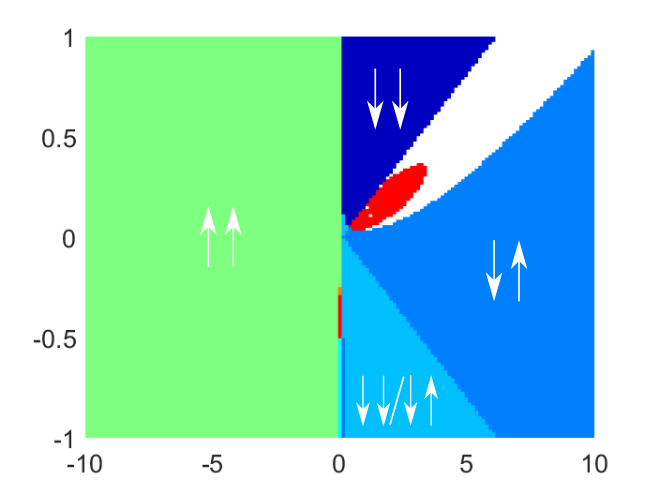
\includegraphics[width=1\textwidth]{Figures/BulkXi0R0.png}};
\node [right=of img,rotate=90,anchor=north,yshift=9.3cm,xshift=0cm] {\large{$J_{\text{RKKY}}$ (mJ/m$^2$)}}; 
\node at (120pt,0pt) {\large{$j_x$ (10$^8$ A/cm$^2$)}};
\end{tikzpicture}
  \caption{$\beta = 0$, $\alpha_\text{R} = 0$ eV$\cdot$m.}
  \label{fig:BulkXi0R0}
\end{subfigure}%
\begin{subfigure}{.49\textwidth}
  \centering
    \begin{tikzpicture}
\node[above right] (img) at (0,0) {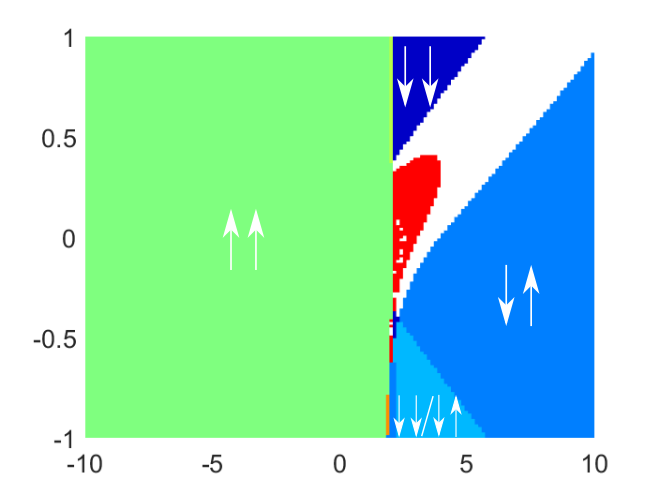
\includegraphics[width=1\textwidth]{Figures/BulkXi0R5v3.png}};
\node [right=of img,rotate=90,anchor=north,yshift=9.3cm,xshift=0cm] {\large{$J_{\text{RKKY}}$ (mJ/m$^2$)}}; 
\node at (120pt,0pt) {\large{$j_x$ (10$^8$ A/cm$^2$)}};
\end{tikzpicture}
  \caption{$\beta = 0$, $\alpha_\text{R} = 1.85\cdot10^{-10}$ eV$\cdot$m.}
  \label{fig:BulkXi0R5}
\end{subfigure}

\begin{subfigure}{.49\textwidth}
  \centering
    \begin{tikzpicture}
\node[above right] (img) at (0,0) {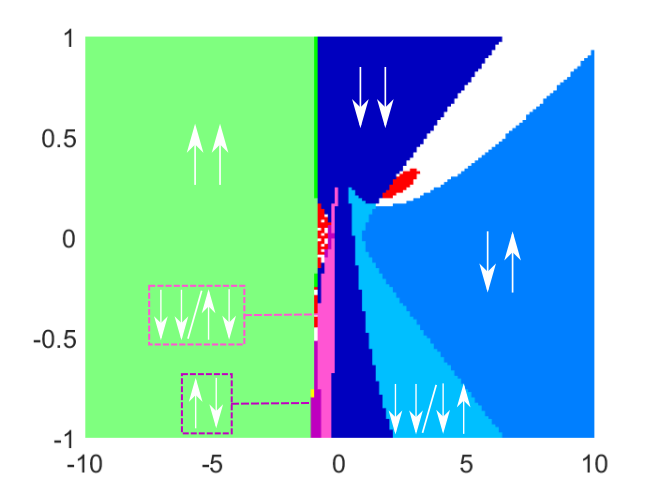
\includegraphics[width=1\textwidth]{Figures/BulkXi15R5v3.png}};
\node [right=of img,rotate=90,anchor=north,yshift=9.3cm,xshift=0cm] {\large{$J_{\text{RKKY}}$ (mJ/m$^2$)}}; 
\node at (120pt,0pt) {\large{$j_x$ (10$^8$ A/cm$^2$)}};
\end{tikzpicture}
  \caption{$\beta = 0.015$, $\alpha_\text{R} = 1.85\cdot10^{-10}$ eV$\cdot$m.}
  \label{fig:BulkXi15R5}
\end{subfigure}%
\begin{subfigure}{.49\textwidth}
  \centering
    \begin{tikzpicture}
\node[above right] (img) at (0,0) {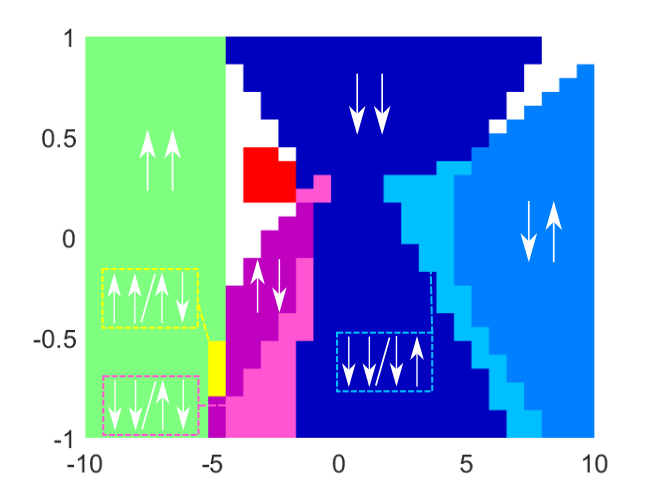
\includegraphics[width=1\textwidth]{Figures/BulkXi15R25v3.png}};
\node [right=of img,rotate=90,anchor=north,yshift=9.3cm,xshift=0cm] {\large{$J_{\text{RKKY}}$ (mJ/m$^2$)}}; 
\node at (120pt,0pt) {\large{$j_x$ (10$^8$ A/cm$^2$)}};
\end{tikzpicture}
  \caption{$\beta = 0.015$, $\alpha_\text{R} = 9.26\cdot10^{-10}$ eV$\cdot$m.}
  \label{fig:BulkXi15R25}
\end{subfigure}
\caption{Phase diagrams for the bulk geometry. For all phase diagrams the values $\alpha=0.01$, $P=0.5$, $j_y=10^9$ A/cm$^2$, $K=8\cdot10^4$ J/m$^3$, $d=3$ nm are assumed. The red regions indicate an STO phase, while the white regions are canted states. }
\label{fig:STOBulkPhase}
\end{figure}
By combining the analytical framework and numerical method described previously, we can create phase diagrams that show for what parameters the different collinear states are stable, when we have an STO phase, and when we are in a canted state. We perform these calculations with the same parameters as Zhou \etal~\cite{Zhou2013} for an easy comparison between the results with and without RSOC. These parameters are $\alpha=0.01$, $P=0.5$, $K=8\cdot10^4$ J/m$^3$, $d=3$ nm, $J \sim 1$ mJ/m$^2$, $j_x\sim 10^8$ A/cm$^2$, $M_s = 127$ kA/m. In the bulk geometry we also set $j_y=10^9$ A/cm$^2$. Regarding the strength of the Rashba parameter $\alpha_{\text{R}}$ we consider the values $\alpha_{\text{R}}=0$, $1.85\cdot10^{-10}$ eV$\cdot$m, $9.26\cdot10^{-10}$ eV$\cdot$m. These rather high values are chosen to get a clear indication of the effects RSOC may have. The values are also chosen not to be unrealistic, as $\alpha_{\text{R}}$ has been found to be $\sim 3.7 \cdot 10^{-10}$ eV$\cdot$m at the surface of Bi/Ag alloy \cite{Manchon2015}. In the bulk geometry the strength of the Rashba parameter is not too important, as we can adjust for a lower $\alpha_{\text{R}}$ by increasing $j_y$ accordingly. This is not possible in the thin film geometry, however, as both spin-transfer torques and RSOC are controlled by the current $j_x$, and so the strength of $\alpha_{\text{R}}$ becomes more important in the thin film geometry. 

Performing the calculations, the resulting phase diagrams for the bulk geometry are shown in Figure \ref{fig:STOBulkPhase}, and the phase diagrams for the thin film geometry are shown in Figure \ref{fig:STOFilmPhase}. The phase diagram without the effects of RSOC, as found by Zhou et al., is presented in Figure \ref{fig:BulkXi0R0}. We see by comparing it to a system with RSOC present, as shown in Figure \ref{fig:BulkXi0R5}, that RSOC can increase the size of the STO phase and even extend it down to the antiferromagnetic regime for compensated magnetic moments $\mathbold{m}_i$. Now to compare our results to our analogy of RSOC effectively modifying the Gilbert damping $\alpha$. According to Zhou \etal~the border between the unstable region (STO phase and the canted state, illustrated in red and white) and the $\uparrow\downarrow$ state is approximately given by
\begin{align}
    \omega_J = \sqrt{4\omega_0^2+\left(\omega_j^{(x)}\right)^2}-2\omega_0+\alpha\frac{\omega_0^2}{\omega_j^{(x)}}.
\end{align}
For $\alpha>0$ we would therefore expect the border to increase as $j_x\rightarrow 0^+$, as in Figure \ref{fig:BulkXi0R0}. In Figure \ref{fig:BulkXi0R5}, however, this border decreases as $j_x\rightarrow 0^+$ as if $\alpha<0$. As we remember from our analogy, we found that the effective Gilbert damping $\Real (\alpha^*)$ could become negative in the presence of RSOC for some set of parameters. This seems to be the case here. We also remember that we could switch from being in a minimal region in $\Real (\alpha^*)$ to a maximal region by letting $\beta>\alpha$ if we were in a minimal region when $\beta<\alpha$. The phase diagram in this case is shown in Figure \ref{fig:BulkXi15R5}. As predicted, the border between the unstable region and the $\uparrow\downarrow$ state is lifted. In addition, the size of the STO phase localized in that region decreases, which would correspond well with an increase in the Gilbert damping. This does not mean systems with $\beta>\alpha$ are of no interest to get an increase in the size of the STO phase, however. We also noted in our analogy that we could also go from being in a minimal to a maximal region in $\Real (\alpha^*)$ by switching the direction of the current in the $y$-direction.
\begin{figure}[h!]
\centering
\begin{subfigure}{.49\textwidth}
  \centering
    \begin{tikzpicture}
\node[above right] (img) at (0,0) {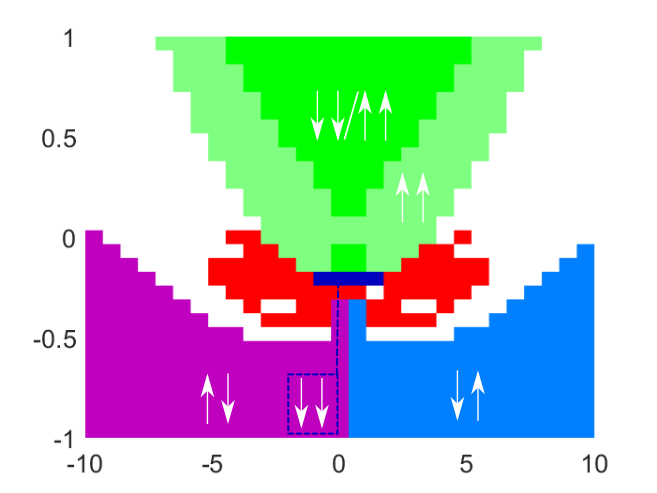
\includegraphics[width=1\textwidth]{Figures/FilmXi0R25v3.png}};
\node [right=of img,rotate=90,anchor=north,yshift=9.3cm,xshift=0cm] {\large{$J_{\text{RKKY}}$ (mJ/m$^2$)}}; 
\node at (120pt,0pt) {\large{$j_x$ (10$^8$ A/cm$^2$)}};
\end{tikzpicture}
  \caption{$\beta = 0$, $\alpha_\text{R} = 9.26\cdot10^{-10}$ eV$\cdot$m.}
  \label{fig:STOFilmXi0R25}
\end{subfigure}%
\begin{subfigure}{.49\textwidth}
  \centering
    \begin{tikzpicture}
\node[above right] (img) at (0,0) {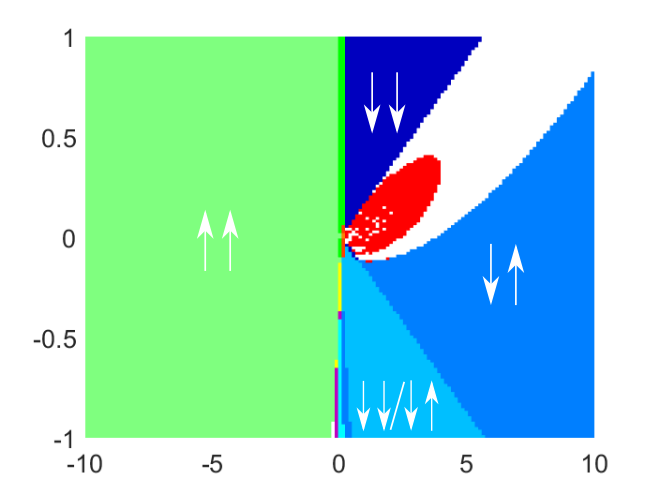
\includegraphics[width=1\textwidth]{Figures/FilmXi05R25v3.png}};
\node [right=of img,rotate=90,anchor=north,yshift=9.3cm,xshift=0cm] {\large{$J_{\text{RKKY}}$ (mJ/m$^2$)}}; 
\node at (120pt,0pt) {\large{$j_x$ (10$^8$ A/cm$^2$)}};
\end{tikzpicture}
  \caption{$\beta = 0.005$, $\alpha_\text{R} = 9.26\cdot10^{-10}$ eV$\cdot$m.}
  \label{fig:STOFilmXi05R25}
\end{subfigure}

\caption{Phase diagrams for the thin film geometry. For all phase diagrams the values $\alpha=0.01$, $P=0.5$, $K=8\cdot10^4$ J/m$^3$, $d=3$ nm are assumed. The red regions indicate an STO phase, while the white regions are canted states. }
\label{fig:STOFilmPhase}
\end{figure}
\begin{figure}[h!]
\centering
\begin{subfigure}{.49\textwidth}
  \centering
    \begin{tikzpicture}
\node[above right] (img) at (0,0) {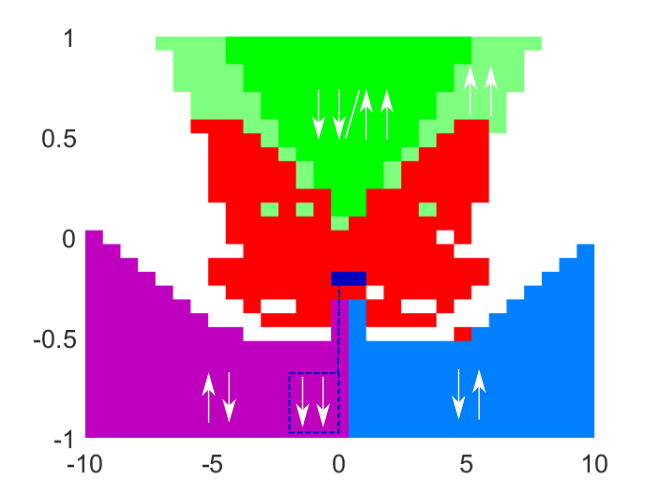
\includegraphics[width=1\textwidth]{Figures/FilmXi0R25ddv3.png}};
\node [right=of img,rotate=90,anchor=north,yshift=9.3cm,xshift=0cm] {\large{$J_{\text{RKKY}}$ (mJ/m$^2$)}}; 
\node at (120pt,0pt) {\large{$j_x$ (10$^8$ A/cm$^2$)}};
\end{tikzpicture}
  \caption{}
  \label{fig:StabilityDD}
\end{subfigure}%
\begin{subfigure}{.49\textwidth}
  \centering
    \begin{tikzpicture}
\node[above right] (img) at (0,0) {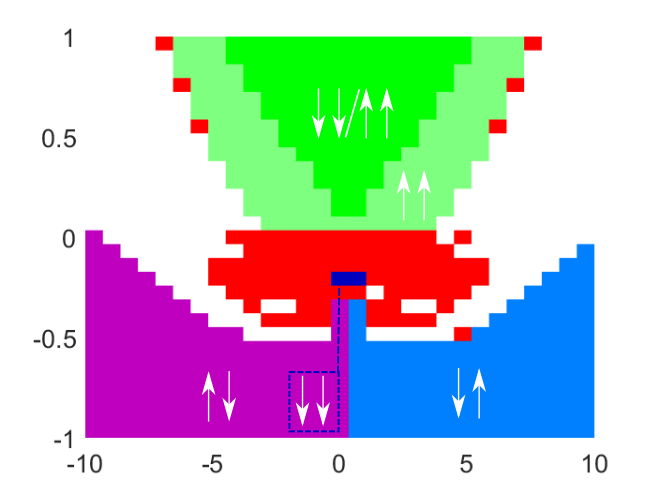
\includegraphics[width=1\textwidth]{Figures/FilmXi0R25uuv3.png}};
\node [right=of img,rotate=90,anchor=north,yshift=9.3cm,xshift=0cm] {\large{$J_{\text{RKKY}}$ (mJ/m$^2$)}}; 
\node at (120pt,0pt) {\large{$j_x$ (10$^8$ A/cm$^2$)}};
\end{tikzpicture}
  \caption{}
  \label{fig:StabilityUU}
\end{subfigure}

\caption{The stability of the $\uparrow\uparrow$ state in the thin film geometry for $\beta = 0$, $\alpha_\text{R} = 9.26\cdot10^{-10}$ eV$\cdot$m is found to be very dependent on the initial conditions. In \textbf{(a)} the initial state is chosen to be close to $\downarrow\downarrow$ for $J_{\text{RKKY}}>0$, while in \textbf{(b)} the initial state is chosen to be close to $\uparrow\uparrow$ in the same region. In both cases the initial state is chosen to be close to $\downarrow\uparrow$ for $J_{\text{RKKY}}<0$.}
\label{fig:STOFilmStability}
\end{figure}

Moving on to the thin film geometry, we get a different behavior in the phase diagrams. We do not get the same behavior in the border between the unstable region and the $\uparrow\downarrow$ state due to the fact that the effects of RSOC are proportional to $j_x$, and as $j_x\rightarrow 0$ these effects vanish. We can, however, still see a lowering of the border with RSOC present, as shown in both Figure \ref{fig:STOFilmXi0R25} and \ref{fig:STOFilmXi05R25}, but we do not have the same effect when $j_x\rightarrow 0^+$. In the phase diagrams shown here we also have an increase in the STO phase for the thin film geometry when RSOC is present, though this increase requires a rather large Rashba parameter $\alpha_{\text{R}}$ to become evident. We are also able to find an STO phase in the antiferromagnetic regime ($J_{\text{RKKY}}<0$), most noticeably in the case with $\beta = 0$, $\alpha_\text{R} = 9.26\cdot10^{-10}$ eV$\cdot$m as illustrated in Figure \ref{fig:STOFilmXi0R25}. This STO phase is also more or less symmetric in $j_x$. Something that should be noted with this set of parameters is that while we have a region where the $\uparrow\uparrow$ state is stable, numerical calculations show that whether the system relaxes to this state is highly dependent on the initial condition of $\mathbold{m}_1$ and $\mathbold{m}_2$. In Figure \ref{fig:STOFilmStability} we show all the points in the phase diagram that are found to be in an oscillating state for different initial conditions. This is in contrast with Figure \ref{fig:STOBulkPhase} and \ref{fig:STOFilmPhase} where we only classify a point to be an oscillating state if the numerical calculations indicate this and the analytical calculations say there are no stable collinear states the system can relax to. In all figures the stability of the collinear states are determined analytically, while the STO phase is found numerically. As we can see in Figure \ref{fig:StabilityDD} an initial condition that is close to $\downarrow\downarrow$ or $\downarrow\uparrow$ does not relax to the $\uparrow\uparrow$ state even if this is stable, and we can also get an STO phase in the ferromagnetic regime. This can be understood by looking at the imaginary component of $\omega$ belonging to the $\uparrow\uparrow$ state for these parameters. It is found that the imaginary component, while less than zero, only has a magnitude of $10^{-2}$. In comparison the other stable regions typically have an order of magnitude up to $10^1$. It is therefore not surprising that if the initial state is far away from being in $\uparrow\uparrow$ it is possible that the system will not relax to that state, and we can get an oscillating or canted state even though there exists a stable collinear state.

The sensitivity issue concerning the initial state of $\mathbold{m}_1$ and $\mathbold{m}_2$ was only of considerable significance for the $\uparrow\uparrow$ state in the thin-film geometry with $\beta = 0$, $\alpha_\text{R} = 9.26\cdot10^{-10}$ eV$\cdot$m. There was also some sensitivity for other phase diagrams in the limit $j_x\rightarrow 0$. Regarding the cutoff factors utilized for classifying the numerical solution, there was very little sensitivity in the choice of parameters. The transitional region between an STO state and a canted or collinear state is found to happen on a typical scale of $10^{6}$ A/cm$^2$ or $10^{-3}$ mJ/m$^2$, both of which being very small compared to the magnitude of the parameters considered. As the cutoff factors would primarily have an effect in this transitional region, a change in these parameters would not lead to a significant change in the size of the STO phase. It can also be seen in some of the phase diagrams that there are found to be some canted states in the middle of the STO region, or a single STO state separated from the main STO region. This is discovered to be due to the time interval the system is solved over, as for some parameters it takes longer time for the system to obtain stable oscillations than for others. The time scale that the system was solved over was constrained to some degree, due to the run-time of the solver. It is also observed that the initial state of $\mathbold{m}_1$ and $\mathbold{m}_2$ has some impact on how fast these oscillations become stable. When solving the system over a longer time scale the STO regions should become more or less continuous.

\begin{figure}[h!]
\centering
\begin{subfigure}{.49\textwidth}
  \centering
    \begin{tikzpicture}
\node[above right] (img) at (0,0) {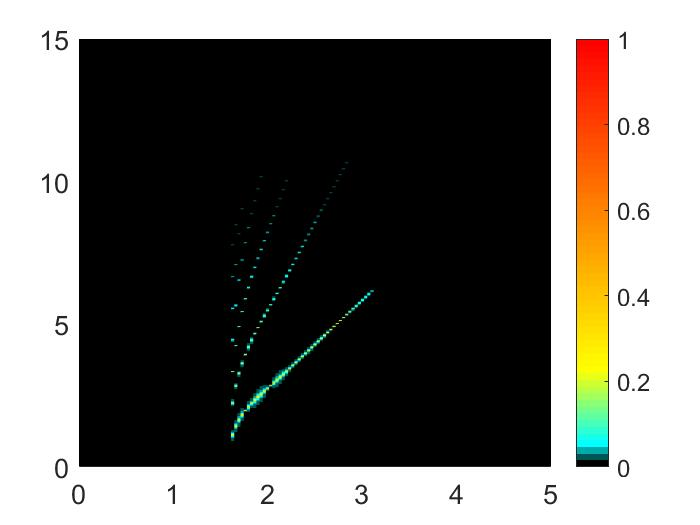
\includegraphics[width=1\textwidth]{Figures/FFT_bulk_xi0R0J025v2.jpg}};
\node [right=of img,rotate=90,anchor=north,yshift=9.3cm,xshift=0cm] {\large{$f$ (GHz)}}; 
\node at (105pt,0pt) {\large{$j_x$ (10$^8$ A/cm$^2$)}};
\end{tikzpicture}
  \caption{$\beta = 0$, $\alpha_\text{R} = 0$ eV$\cdot$m.}
\end{subfigure}%
\begin{subfigure}{.49\textwidth}
  \centering
    \begin{tikzpicture}
\node[above right] (img) at (0,0) {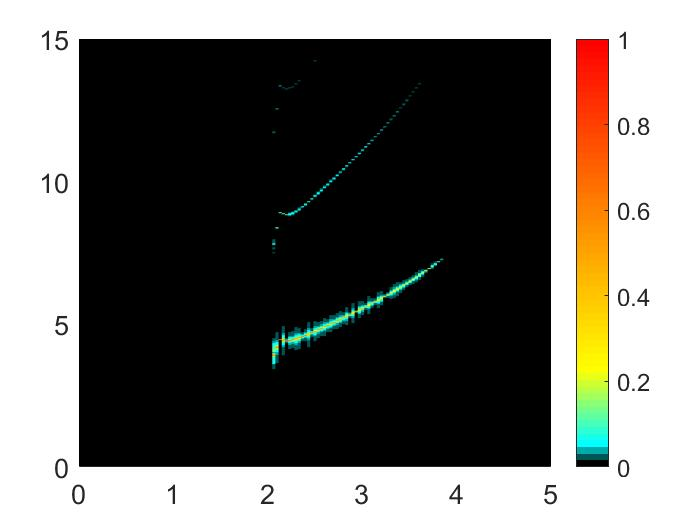
\includegraphics[width=1\textwidth]{Figures/FFT_bulk_xi0R5J025v2.jpg}};
\node [right=of img,rotate=90,anchor=north,yshift=9.3cm,xshift=0cm] {\large{$f$ (GHz)}}; 
\node at (105pt,0pt) {\large{$j_x$ (10$^8$ A/cm$^2$)}};
\end{tikzpicture}
  \caption{$\beta = 0$, $\alpha_\text{R} = 1.85\cdot10^{-10}$ eV$\cdot$m.}
  \label{fig:FFTBulkXi0R5}
\end{subfigure}

\begin{subfigure}{.49\textwidth}
  \centering
    \begin{tikzpicture}
\node[above right] (img) at (0,0) {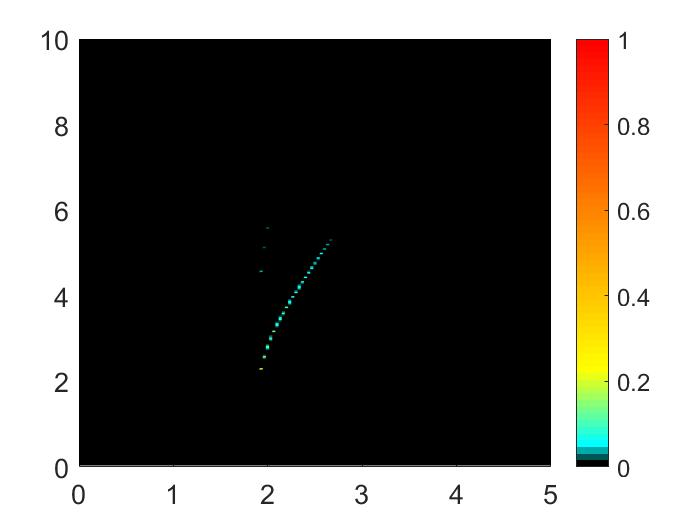
\includegraphics[width=1\textwidth]{Figures/FFT_bulk_xi15R5J025v2.jpg}};
\node [right=of img,rotate=90,anchor=north,yshift=9.3cm,xshift=0cm] {\large{$f$ (GHz)}}; 
\node at (105pt,0pt) {\large{$j_x$ (10$^8$ A/cm$^2$)}};
\end{tikzpicture}
  \caption{$\beta = 0.005$, $\alpha_\text{R} = 1.85\cdot10^{-10}$ eV$\cdot$m.}
  \label{fig:FFTBulkXi15R5}
\end{subfigure}
\begin{subfigure}{.49\textwidth}
  \centering
    \begin{tikzpicture}
\node[above right] (img) at (0,0) {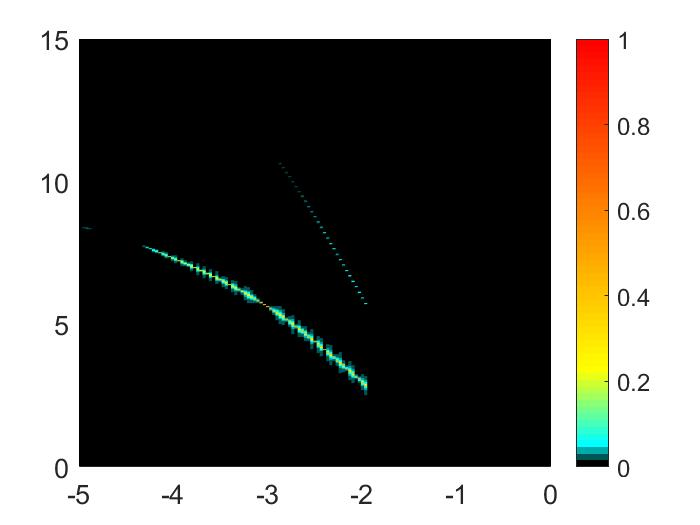
\includegraphics[width=1\textwidth]{Figures/FFT_bulk_xi15R25J025v2.jpg}};
\node [right=of img,rotate=90,anchor=north,yshift=9.3cm,xshift=0cm] {\large{$f$ (GHz)}}; 
\node at (105pt,0pt) {\large{$j_x$ (10$^8$ A/cm$^2$)}};
\end{tikzpicture}
  \caption{$\beta = 0.015$, $\alpha_\text{R} = 9.26\cdot10^{-10}$ eV$\cdot$m.}
  \label{fig:FFTBulkXi15R25}
\end{subfigure}

\caption{The one sided spectra of the Fourier transform of $\mathbold{m}_0\cdot\mathbold{m}_1$ in the bulk geometry. The Fourier transform was taken along the $J_{\text{RKKY}}=0.25$ mJ/m$^2$ line in the phase diagrams.}
\label{fig:STOBulkFreq}
\end{figure}
\subsection{Frequency spectra}
We have now shown that with the presence of RSOC we are able to increase the size of the STO phase. It is also of interest to study what impact RSOC has on the frequency spectrum. To study this we take fast Fourier transforms of $\mathbold{m}_0\cdot\mathbold{m}_1$ for selected values of $J_{\text{RKKY}}$. The Fourier transforms of $\mathbold{m}_1\cdot\mathbold{m}_2$ are not presented as they show the same frequency spectra, but with slightly different amplitudes. The results for the bulk geometry are shown in Figure \ref{fig:STOBulkFreq}, and the results for the thin film geometry are shown in Figure \ref{fig:STOFilmFreq}. First considering the results from the bulk geometry, we see that in the presence of RSOC we have fewer frequencies for a given $j_x$ in comparison to the case without RSOC. Moreover, we see that the amplitude of the oscillations can also be larger when we have RSOC in the system, as seen in Figure \ref{fig:FFTBulkXi0R5} and \ref{fig:FFTBulkXi15R25}. For some parameters they can also be smaller, however, as seen in Figure \ref{fig:FFTBulkXi15R5}. The main frequency in the presence of RSOC tends to be more slowly varying as a function of $j_x$ than the system without RSOC, but we can obtain slightly higher frequencies with RSOC than without. In addition, the oscillations in the presence of RSOC can also have higher amplitudes than the system without RSOC, as shown in Figure \ref{fig:FFTBulkXi0R5} and \ref{fig:FFTBulkXi15R25}. As the strength of RSOC is controllable by $j_y$, this allows for a more tunable frequency spectrum in the spin torque oscillator when the effects of RSOC are included. We now have two parameters we can vary to control the frequency output without changing the materialistic properties instead of just one.

Considering the frequency spectra in the thin film geometry we see that for the ferromagnetically coupled magnetic moments in Figure \ref{fig:FFTFilmXi05R25} the behavior is rather similar to the bulk geometry case in Figure \ref{fig:FFTBulkXi0R5}. We have higher amplitudes of the oscillations, and a reduction in the amount of frequencies. The frequency as a function of current is slightly steeper than in the bulk geometry, however. The result that makes the thin film geometry stand out from the bulk geometry is the frequency spectrum of the antiferromagnetically coupled magnetic moments in Figure \ref{fig:FFTFilmXi0R25}. As we can see, the frequency spectrum reflects the same symmetry in $j_x$ as the STO phase in the phase diagram. In addition, we have several more frequencies available in this antiferromagnetic STO than in the ferromagnetic STO.
\begin{figure}[h!]
\centering
\begin{subfigure}{.49\textwidth}
  \centering
    \begin{tikzpicture}
\node[above right] (img) at (0,0) {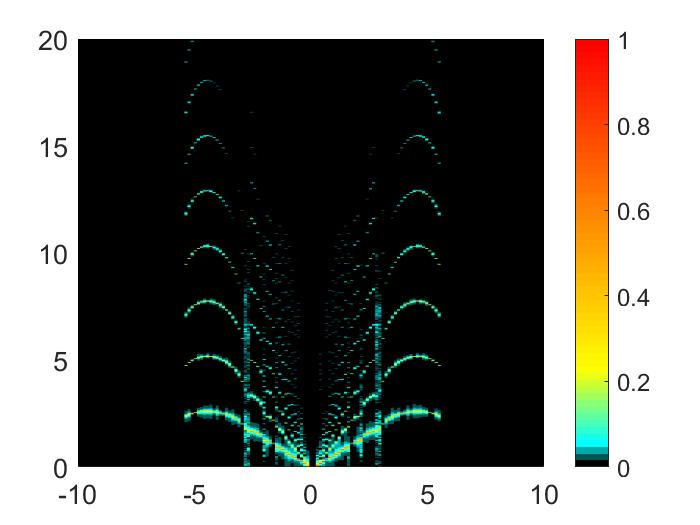
\includegraphics[width=1\textwidth]{Figures/FFT_film_xi0R25Jn02v2.jpg}};
\node [right=of img,rotate=90,anchor=north,yshift=9.3cm,xshift=0cm] {\large{$f$ (GHz)}}; 
\node at (105pt,0pt) {\large{$j_x$ (10$^8$ A/cm$^2$)}};
\end{tikzpicture}
  \caption{$\beta = 0$, $\alpha_\text{R} = 9.26\cdot10^{-10}$ eV$\cdot$m.}
  \label{fig:FFTFilmXi0R25}
\end{subfigure}%
\begin{subfigure}{.49\textwidth}
  \centering
    \begin{tikzpicture}
\node[above right] (img) at (0,0) {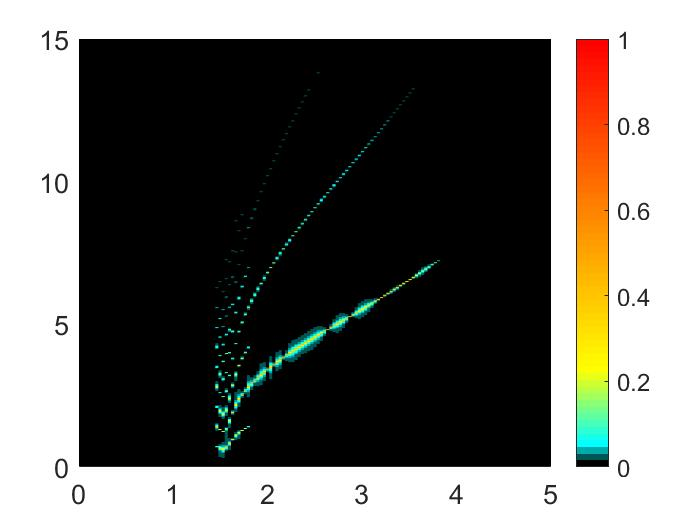
\includegraphics[width=1\textwidth]{Figures/FFT_film_xi05R25J025v2.jpg}};
\node [right=of img,rotate=90,anchor=north,yshift=9.3cm,xshift=0cm] {\large{$f$ (GHz)}}; 
\node at (105pt,0pt) {\large{$j_x$ (10$^8$ A/cm$^2$)}};
\end{tikzpicture}
  \caption{$\beta = 0.005$, $\alpha_\text{R} = 9.26\cdot10^{-10}$ eV$\cdot$m.}
  \label{fig:FFTFilmXi05R25}
\end{subfigure}

\caption{The one sided spectra of the Fourier transform of $\mathbold{m}_0\cdot\mathbold{m}_1$ in the thin film geometry. The Fourier transform was taken along the $J_{\text{RKKY}}=-0.2$ mJ/m$^2$ line in \textbf{(a)} and along $J_{\text{RKKY}}=0.25$ mJ/m$^2$ in \textbf{(b)}.}
\label{fig:STOFilmFreq}
\end{figure}